You are given the following data situation:
\begin{knitrout}
\definecolor{shadecolor}{rgb}{0.969, 0.969, 0.969}\color{fgcolor}\begin{kframe}
\begin{alltt}
\hlkwd{library}\hlstd{(ggplot2)}

\hlkwd{set.seed}\hlstd{(}\hlnum{314}\hlstd{)}
\hlstd{n} \hlkwb{<-} \hlnum{100}
\hlstd{X} \hlkwb{=} \hlkwd{cbind}\hlstd{(}\hlkwd{rnorm}\hlstd{(n,} \hlopt{-}\hlnum{5}\hlstd{,} \hlnum{5}\hlstd{),}
  \hlkwd{rnorm}\hlstd{(n,} \hlopt{-}\hlnum{10}\hlstd{,} \hlnum{10}\hlstd{))}
\hlstd{X_design} \hlkwb{=} \hlkwd{cbind}\hlstd{(}\hlnum{1}\hlstd{, X)}

\hlstd{z} \hlkwb{<-} \hlnum{2}\hlopt{*}\hlstd{X[,}\hlnum{1}\hlstd{]} \hlopt{+} \hlnum{3}\hlopt{*}\hlstd{X[,}\hlnum{2}\hlstd{]}
\hlstd{pr} \hlkwb{<-} \hlnum{1}\hlopt{/}\hlstd{(}\hlnum{1}\hlopt{+}\hlkwd{exp}\hlstd{(}\hlopt{-}\hlstd{z))}
\hlstd{y} \hlkwb{<-} \hlkwd{as.integer}\hlstd{(pr} \hlopt{>} \hlnum{0.5}\hlstd{)}
\hlstd{df} \hlkwb{<-} \hlkwd{data.frame}\hlstd{(}\hlkwc{X} \hlstd{= X,} \hlkwc{y} \hlstd{= y)}

\hlkwd{ggplot}\hlstd{(df)} \hlopt{+}
  \hlkwd{geom_point}\hlstd{(}\hlkwd{aes}\hlstd{(}\hlkwc{x} \hlstd{= X.1,} \hlkwc{y} \hlstd{= X.2,} \hlkwc{color}\hlstd{=y))} \hlopt{+}
  \hlkwd{xlab}\hlstd{(}\hlkwd{expression}\hlstd{(theta[}\hlnum{1}\hlstd{]))} \hlopt{+}
  \hlkwd{ylab}\hlstd{(}\hlkwd{expression}\hlstd{(theta[}\hlnum{2}\hlstd{]))}
\end{alltt}
\end{kframe}
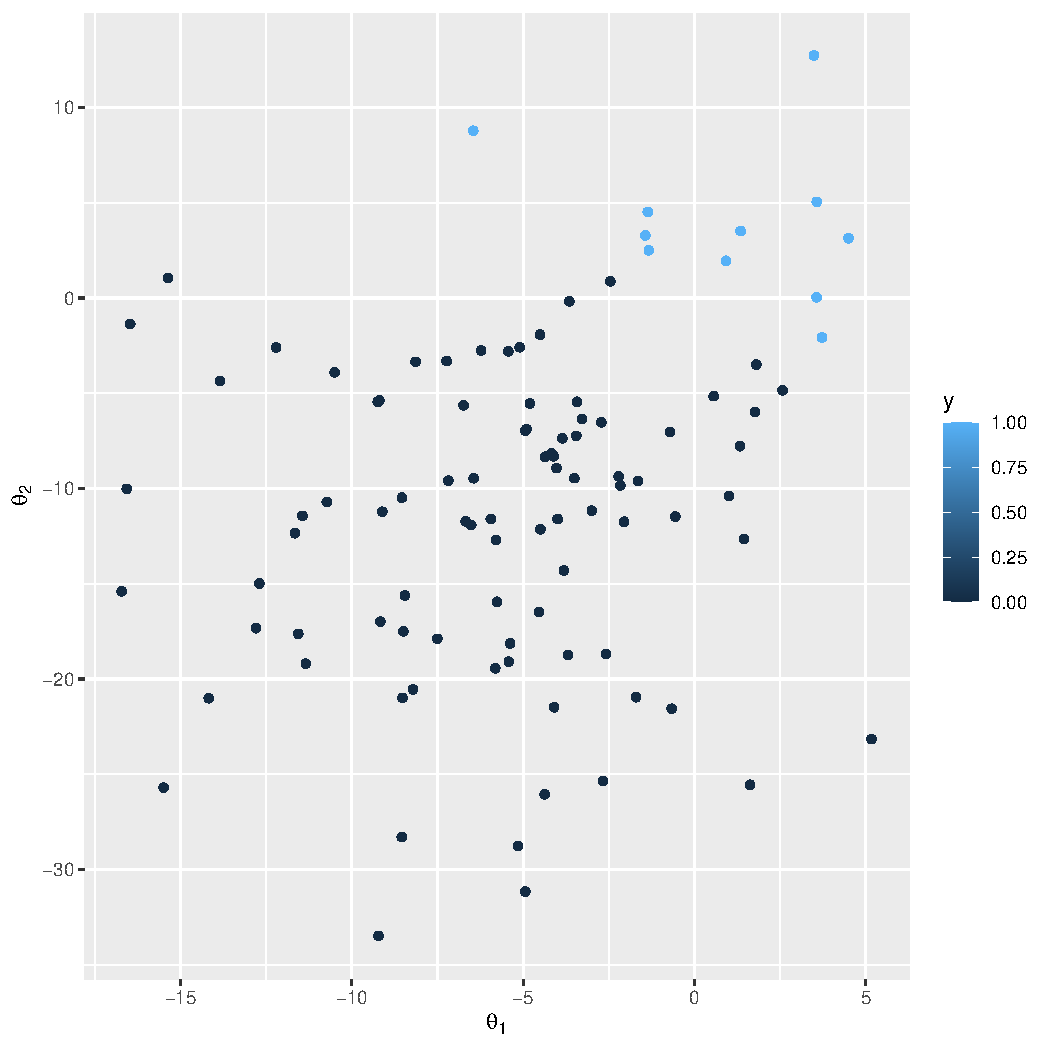
\includegraphics[width=0.5\linewidth]{figure/mv-plot-1} 
\end{knitrout}

In the following we want to estimate a logistic regression without intercept via gradient descent\footnote{We chose this algorithm for educational purposes; in practice, we typically use second order algorithms.}.
\begin{enumerate}
\item  
First consider the derivative of $g:\R \rightarrow \R, z\mapsto \log(1+\exp(z)) - z$, i.e.,\\
$g'(z) = \underbrace{\frac{\exp(z)}{1+\exp(z)}}_{< 1} - 1 < 0 \Rightarrow g$ is monotonically decreasing $\Rightarrow g(z) > g(\alpha z) \quad \forall z \in \R$ and $\alpha > 0.$
\\
Second consider the derivative of $h:\R \rightarrow \R, z\mapsto \log(1+\exp(-z))$, i.e.,\\
$h'(z) = -\underbrace{\frac{\exp(z)}{1+\exp(z)}}_{>0} < 0 \Rightarrow h$ is monotonically decreasing $\Rightarrow h(z) > h(\alpha z) \quad \forall z \in \R$ and $\alpha > 0.$

With this we get \\
$\mathcal{R}_\text{emp}(\tilde{\bm{\theta}}) = \sum^n_{i=1} \log(1 + \exp(\tilde{\bm{\theta}}^\top \mathbf{x}^{(i)})) - y^{(i)}\tilde{\bm{\theta}}^\top \mathbf{x}^{(i)} =$\\
$\sum^n_{i=1} (\mathds{1}_{y^{(i)} = 1} \log(1 + \exp(\vert\tilde{\bm{\theta}}^\top \mathbf{x}^{(i)}\vert)) - \vert\tilde{\bm{\theta}}^\top \mathbf{x}^{(i)}\vert) .$ \\


The data situation is called complete separation, i.e., the classes can be perfectly classified with a linear classifier. Show that in this situation if $\tilde{\bm{\theta}}$ perfectly classifies the data then:\\
$\mathcal{R}_\text{emp}(\tilde{\bm{\theta}}) \geq \mathcal{R}_\text{emp}(\alpha \tilde{\bm{\theta}})$ with $\alpha > 0.$
\item Visualize $\mathcal{R}_\text{emp}$ in $[-1,4]\times[-1,4].$
\item Find the gradient of $\mathcal{R}_\text{emp}$ for arbitrary $\bm{\theta}.$
\item Solve the logistic regression via gradient descent. Use step width $\alpha = 0.01$, starting point $\bm{\theta}^{[0]} = (0,0)^\top$ and train for 500 steps. Repeat this with $\alpha = 0.02$. Explain your observation.\\
\textit{Hint:} a)
\item Repeat d) but add an L2 penalization term (with $\lambda = 1$) to the objective. What do you observe now?
\item Visualize the regularized $\mathcal{R}_\text{emp}$ in $[-1,4]\times[-1,4].$
\item Repeat e) but with backtracking. Set $\gamma = 0.9$ and $\tau = 0.5$
\end{enumerate}
